% =====================================================================
%  Poster: Model-Free PID Tuning via Encirclements of the Step Response
%  A0 portrait (841 x 1189 mm).  Compile with pdflatex (twice).
%  Self-contained: only standard TeX Live packages, no poster class.
% =====================================================================
\documentclass[final]{article}

\usepackage[utf8]{inputenc}
\usepackage[T1]{fontenc}
\usepackage[paperwidth=841mm,paperheight=1189mm,margin=22mm]{geometry}
\usepackage{mathpazo}                 % Palatino text + matched math
\usepackage[scaled=0.92]{helvet}      % Helvetica for headings
\usepackage{xcolor}
\usepackage{graphicx}
\usepackage{booktabs}
\usepackage{tcolorbox}
\usepackage{tikz}
\usepackage{amsmath,amssymb}
\usepackage{enumitem}
\usepackage{microtype}
\tcbuselibrary{skins}
\usetikzlibrary{arrows.meta,positioning}

\pagestyle{empty}
\parindent=0pt
\setlength{\parskip}{0.4\baselineskip}

% ------------------------------------------------------------------ %
\definecolor{ink}      {HTML}{16191D}
\definecolor{navy}     {HTML}{123A5E}
\definecolor{steel}    {HTML}{3C6E9F}
\definecolor{rust}     {HTML}{B23A2E}
\definecolor{paper}    {HTML}{F4F2ED}
\definecolor{panel}    {HTML}{FFFFFF}
\definecolor{rule}     {HTML}{D8D3C8}
\definecolor{tintblue} {HTML}{E8F0F6}
\definecolor{tintred}  {HTML}{FAEBE7}
\definecolor{muted}    {HTML}{5C6470}

\pagecolor{paper}
\color{ink}

% ------------------------------ type scale (A0) -------------------- %
\renewcommand{\normalsize}  {\fontsize{33.5}{42}\selectfont}
\renewcommand{\small}       {\fontsize{29}{36}\selectfont}
\renewcommand{\footnotesize}{\fontsize{26}{32}\selectfont}
\renewcommand{\scriptsize}  {\fontsize{18}{23}\selectfont}
\renewcommand{\large}       {\fontsize{34}{41}\selectfont}
\renewcommand{\Large}       {\fontsize{40}{48}\selectfont}
\renewcommand{\LARGE}       {\fontsize{50}{58}\selectfont}
\renewcommand{\huge}        {\fontsize{64}{74}\selectfont}
\renewcommand{\Huge}        {\fontsize{88}{98}\selectfont}
\normalsize

\newcommand{\sffam}{\fontfamily{phv}\selectfont}
\newcommand{\titlesize}{\fontsize{84}{95}\selectfont}

% ------------------------------ panels ----------------------------- %
\newtcolorbox{panelbox}[1]{
  enhanced,
  colback=panel, colframe=rule, boxrule=0.8pt, arc=3mm,
  left=10mm, right=10mm, top=9mm, bottom=9mm,
  toptitle=3mm, bottomtitle=3mm,
  title={\sffam\bfseries\large #1},
  coltitle=white, colbacktitle=navy,
  attach boxed title to top left={xshift=7mm, yshift=-4mm},
  boxed title style={colframe=navy, arc=1.5mm, left=6mm, right=6mm,
                     top=2.5mm, bottom=2.5mm},
  before skip=0mm, after skip=10mm
}

\newtcolorbox{callout}[1][tintblue]{
  enhanced, colback=#1, colframe=#1, boxrule=0pt, arc=2mm,
  left=7mm, right=7mm, top=5mm, bottom=5mm,
  before skip=4mm, after skip=1mm
}

\newcommand{\coltitlebar}[1]{%
  \begin{tcolorbox}[enhanced, colback=navy, colframe=navy, boxrule=0pt,
                    arc=2mm, left=6mm, right=6mm, top=4mm, bottom=4mm,
                    before skip=0mm, after skip=6mm]
  \color{white}\sffam\bfseries\Large #1
  \end{tcolorbox}}

\setlist[itemize]{leftmargin=10mm, itemsep=5mm, topsep=3mm,
                  parsep=0mm,
                  label=\textcolor{steel}{\rule[0.28em]{9pt}{3pt}}}

\newlength{\colw}
\setlength{\colw}{0.316\textwidth}
\newcommand{\colgap}{\hfill}

% ===================================================================== %
\begin{document}

% --------------------------- HEADER --------------------------------- %
% Logos (optional): the \makebox[0pt] wrappers park them at the far edges
% without taking any width away from the title block.
\noindent
\makebox[0pt][l]{\raisebox{-20mm}{%
% \includegraphics[height=44mm]{logo_uceeb.pdf}
}}%
\begin{minipage}[c]{\textwidth}
\begin{center}
{\sffam\bfseries\titlesize Model-Free PID Tuning by Step-Response Inspection}

\vspace{4mm}
{\large\itshape One ordinary setpoint step tells you \emph{which} of the
three gains is wrong --- no model, no relay test, no optimization.}


\vspace{5mm}
{\Large Daniel Pachner \quad\textcolor{rule}{\textbf{|}}\quad
 Pavel Otta \quad\textcolor{rule}{\textbf{|}}\quad
 Ji\v{r}\'{\i} Dost\'al \quad\textcolor{rule}{\textbf{|}}\quad
 Vladim\'{\i}r Havlena}

\vspace{3mm}
{\small\color{muted} University Centre for Energy Efficient Buildings
 \,\textperiodcentered\, Faculty of Electrical Engineering
 \,\textperiodcentered\, Czech Technical University in Prague}
\end{center}
\end{minipage}%
\makebox[0pt][r]{\raisebox{-20mm}{%
% \includegraphics[height=44mm]{logo_cvut.pdf}
}}

\vspace{3mm}
{\color{navy}\rule{\textwidth}{2.5pt}}
\vspace{3mm}

% --------------------------- COLUMNS -------------------------------- %
\noindent
% =================== COLUMN 1 ======================================= %
\begin{minipage}[t]{\colw}

\coltitlebar{1 \; The question}

\begin{panelbox}{A loop is ringing. Which gain did it?}
\centering
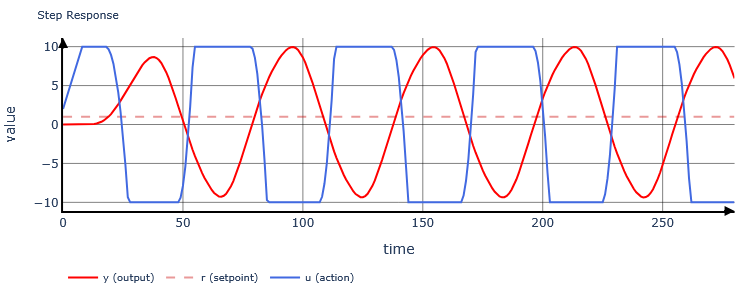
\includegraphics[width=\linewidth]{init_step.png}

\vspace{3mm}
\raggedright
The actuator slams between its limits and the loop never settles.
Nothing here says \emph{which} of the three gains is to blame.

\begin{callout}[tintred]
\sffam\bfseries A step response says \emph{that} the loop is bad.\\
It does not say \emph{what to change}.
\end{callout}
\end{panelbox}

\coltitlebar{2 \; The trick}

\begin{panelbox}{Watch the shape, not the clock}
Plot the error against \emph{itself}. One recorded step, three
pictures --- \textbf{Pachner plots}:

\vspace{1mm}
\begin{center}
\begin{tabular}{@{}ll@{}}
$\Gamma_0$ : & (error,\ accumulated error)\\[2mm]
$\Gamma_1$ : & (change of error,\ error)\\[2mm]
$\Gamma_2$ : & (change of change,\ change of error)
\end{tabular}
\end{center}

\vspace{1mm}
Then \textbf{count the turns around the settling point}. That count is
the \textbf{turn index} $N$. The method:
\mbox{\textbf{S}tep-response} \mbox{\textbf{P}hase-portrait}
\mbox{\textbf{IN}spection} --- \textbf{SPIN}.

\vspace{4mm}
\begin{center}
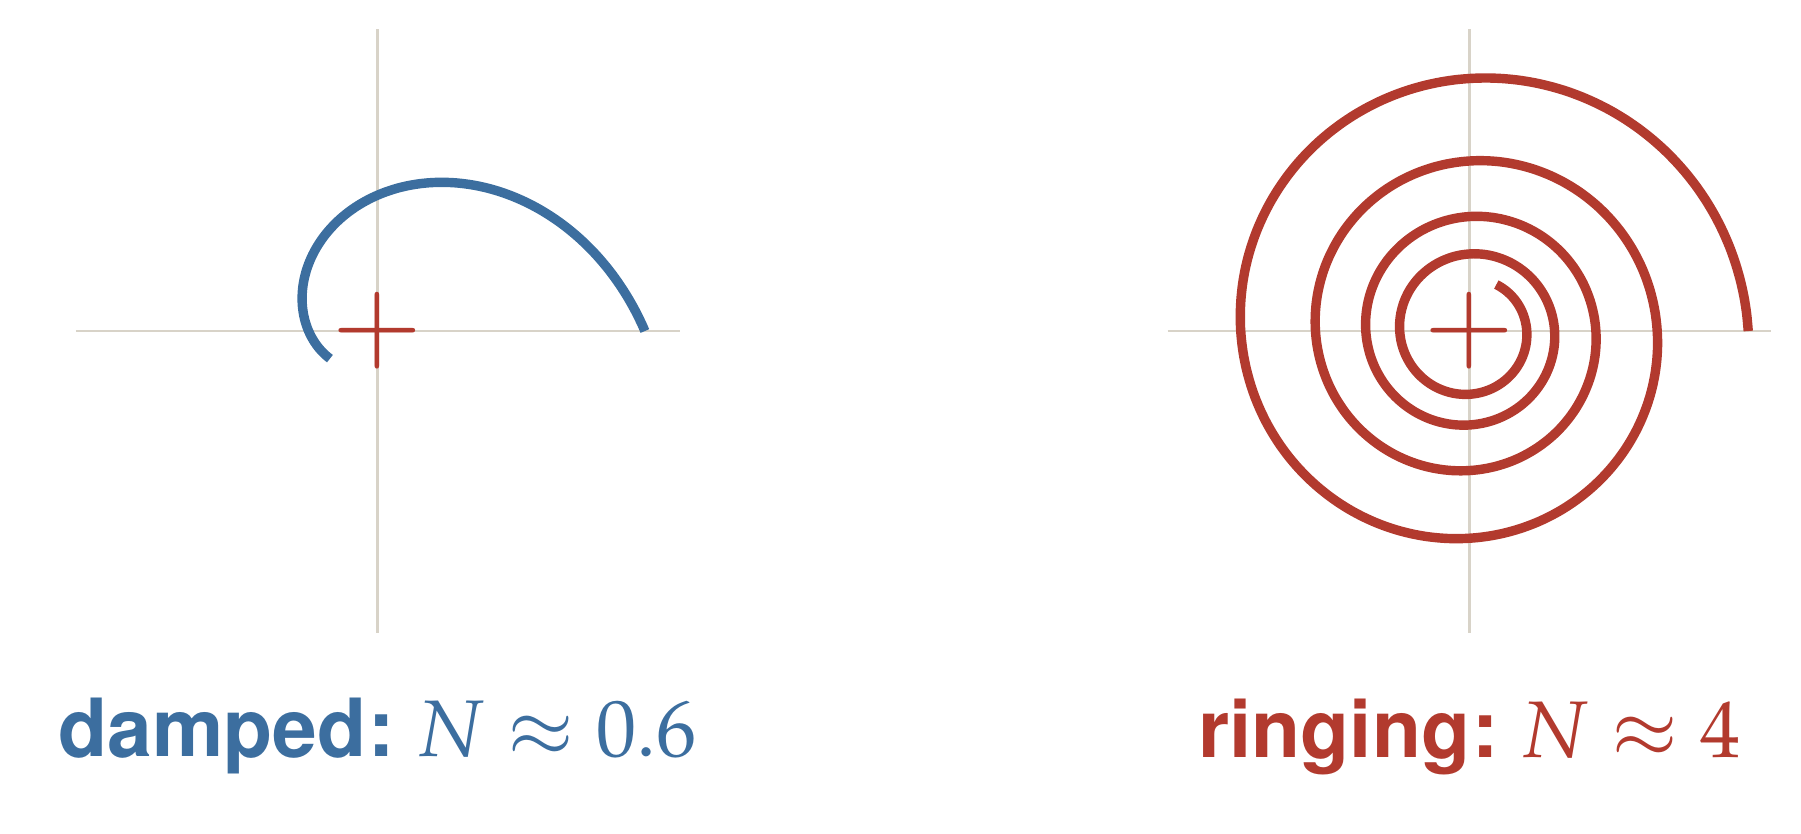
\begin{tikzpicture}[scale=2.95]
  \begin{scope}[shift={(-2.35,0)}]
    \draw[rule, line width=1pt] (-1.3,0) -- (1.3,0);
    \draw[rule, line width=1pt] (0,-1.3) -- (0,1.3);
    \draw[steel, line width=3.4pt, smooth, samples=160]
      plot[domain=0:210, variable=\t]
      ({1.15*exp(-0.0075*\t)*cos(\t)}, {1.15*exp(-0.0075*\t)*sin(\t)});
    \node[rust, font=\bfseries] at (0,0) {\Large $+$};
    \node[anchor=north, font=\small\sffam\bfseries, text=steel]
      at (0,-1.45) {damped:\ $N \approx 0.6$};
  \end{scope}
  \begin{scope}[shift={(2.35,0)}]
    \draw[rule, line width=1pt] (-1.3,0) -- (1.3,0);
    \draw[rule, line width=1pt] (0,-1.3) -- (0,1.3);
    \draw[rust, line width=3.4pt, smooth, samples=420]
      plot[domain=0:1500, variable=\t]
      ({1.2*exp(-0.0011*\t)*cos(\t)}, {1.2*exp(-0.0011*\t)*sin(\t)});
    \node[rust, font=\bfseries] at (0,0) {\Large $+$};
    \node[anchor=north, font=\small\sffam\bfseries, text=rust]
      at (0,-1.45) {ringing:\ $N \approx 4$};
  \end{scope}
\end{tikzpicture}
\end{center}

\vspace{5mm}
\begin{callout}
\sffam\bfseries The turn index has no units.\par
\normalfont\small Independent of step size, of process speed and --- for
fast enough sampling --- of the sampling rate. So one threshold triple
serves every loop: $\bar{\mathbf N} = (0.5,\ 0.75,\ 1.0)$.
\end{callout}
\end{panelbox}

\begin{panelbox}{The three plots of that loop}
\centering
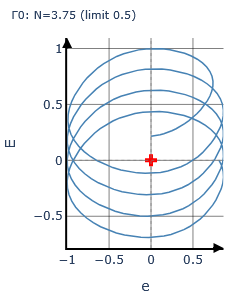
\includegraphics[width=0.325\linewidth]{init_F0.png}\hfill
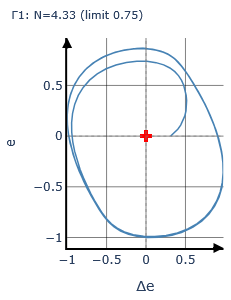
\includegraphics[width=0.325\linewidth]{init_F1.png}\hfill
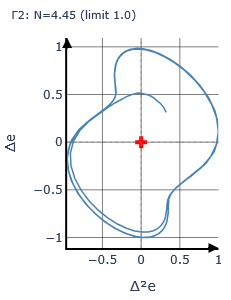
\includegraphics[width=0.325\linewidth]{init_F2.png}

\vspace{3mm}
\raggedright
Counts \textcolor{rust}{$3.75$}, \textcolor{rust}{$4.33$},
\textcolor{rust}{$4.45$} against $0.5$, $0.75$, $1.0$. The fault
invisible above is explicit here --- in every band.
\end{panelbox}

\begin{panelbox}{Where it applies}
\textbf{Yes:} stable, self-regulating processes, with or without dead
time --- heat exchangers, flows, temperatures. Controller I, PI or PID,
integral action present.

\vspace{2mm}
\textbf{No:} integrating or runaway plants, and genuine inverse response
--- on the order of one loop in a hundred.
\end{panelbox}

\end{minipage}
\colgap
% =================== COLUMN 2 ======================================= %
\begin{minipage}[t]{\colw}

\coltitlebar{3 \; Why it names the culprit}

\begin{panelbox}{Each picture hears one speed}
\vspace{1mm}
\begin{center}
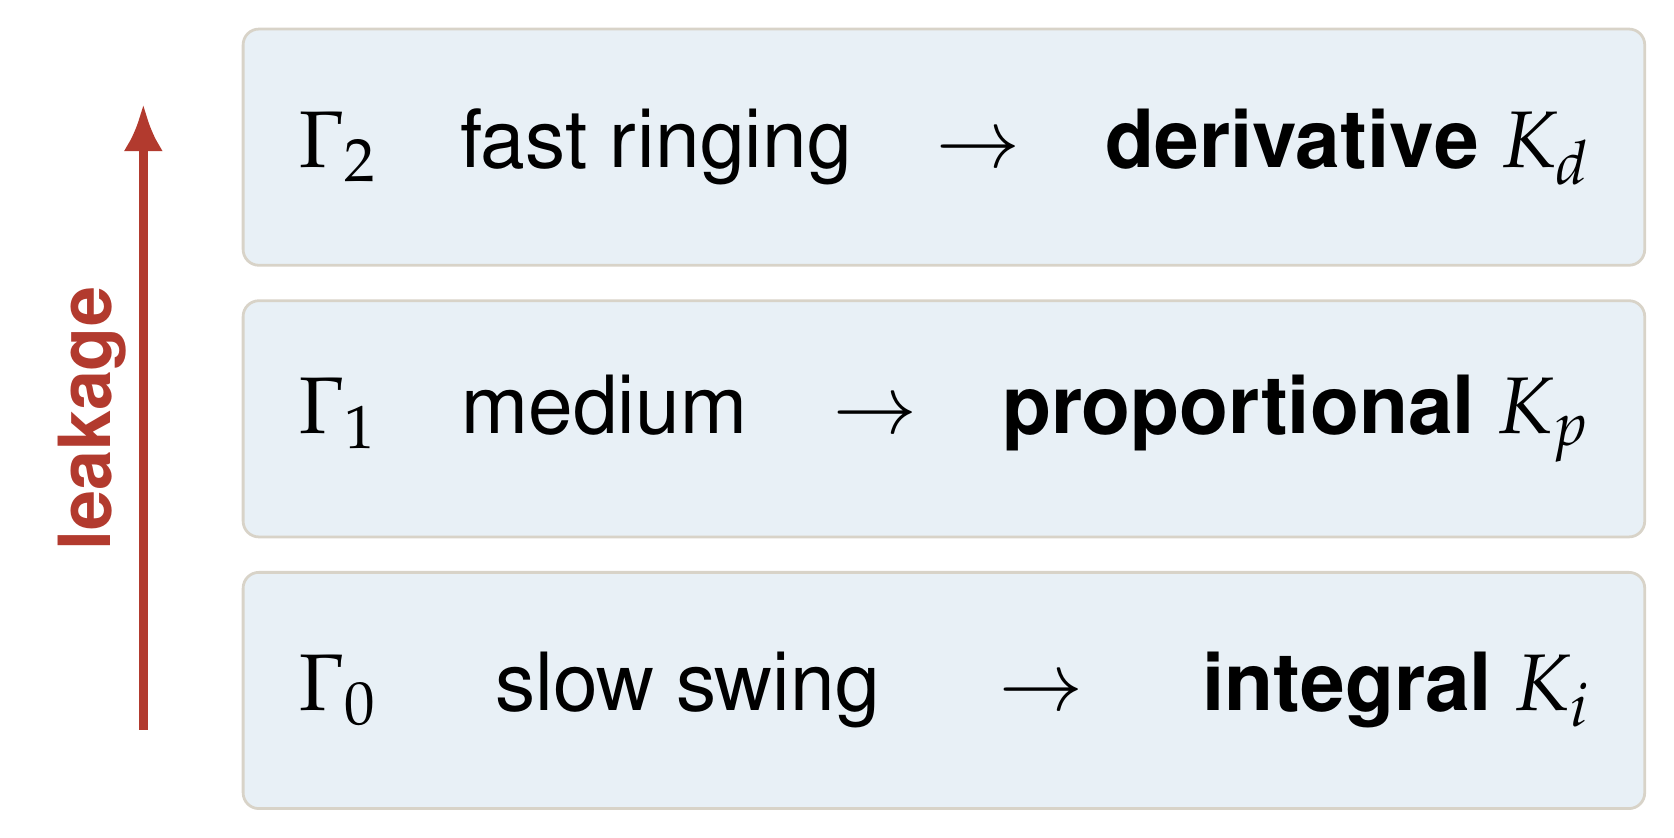
\begin{tikzpicture}[font=\small\sffam]
  \foreach \y/\g/\spd/\lab in {
     0/{$\Gamma_2$}/{fast ringing}/{derivative $K_d$},
     1/{$\Gamma_1$}/{medium}/{proportional $K_p$},
     2/{$\Gamma_0$}/{slow swing}/{integral $K_i$}} {
    \node[draw=rule, line width=1pt, fill=tintblue, rounded corners=2mm,
          minimum width=178mm, minimum height=30mm, anchor=west,
          inner xsep=6mm]
          (b\y) at (2.1,-\y*3.45) {\makebox[164mm][s]{%
            \textbf{\g}\hfill \spd \hfill$\rightarrow$\hfill \textbf{\lab}}};
  }
  \draw[-{Latex[length=6mm,width=5mm]}, rust, line width=3.4pt]
        (0.85,-7.4) -- (0.85,0.55);
  \node[text=rust, font=\footnotesize\sffam\bfseries, rotate=90]
        at (0.2,-3.45) {leakage};
\end{tikzpicture}
\end{center}

\vspace{3mm}
Differencing amplifies fast wiggles, accumulation suppresses them. A slow
fault therefore leaks \emph{upward} into the faster pictures --- but a
fast one never leaks down.

\begin{callout}
\centering\sffam\bfseries\large
The \emph{lowest} violated band is the real fault.\\
Everything above it may be an echo.
\end{callout}
\end{panelbox}

\coltitlebar{4 \; The whole algorithm}

\begin{panelbox}{One table. Nothing else.}
\centering
\renewcommand{\arraystretch}{2.2}
\begin{tabular}{@{}p{0.46\linewidth}p{0.45\linewidth}@{}}
\toprule
\sffam\bfseries the counts say & \sffam\bfseries the tuner does\\
\midrule
never settles                  & halve \emph{all three}\\
lowest is $\Gamma_0$ (slow)    & cut $K_i$\\
lowest is $\Gamma_1$           & cut $K_p$, raise $K_i$\\
lowest is $\Gamma_2$ (fast)    & cut $K_d$, raise $K_p, K_i$\\
nobody complains               & raise \emph{all three}\\
\bottomrule
\end{tabular}

\vspace{5mm}
\raggedright
One notch is about $10\,\%$ of a gain. Then step the setpoint and repeat.
With the violated set $V=\{k : N_k > \bar N_k\}$ and its lowest member
$k_{\min}$,
\vspace{-1mm}
\begin{equation*}
F^{(k)} \leftarrow
\begin{cases}
\gamma\,F^{(k)}, & k < k_{\min} \ \text{(raise)}\\
F^{(k)}/\gamma,  & k = k_{\min} \ \text{(cut)}\\
F^{(k)},         & k > k_{\min} \ \text{(leave)}
\end{cases}
\end{equation*}
\end{panelbox}

\begin{panelbox}{Guaranteed}
\begin{itemize}
\item Ends at the \textbf{largest well-damped gains}, then cycles one
      notch about that boundary.
\item \textbf{Safe from any start}: a diverging record is halved before
      any count is read.
\item \textbf{No guessing}: no model, no relay, no cost function --- the
      move is a table lookup.
\item \textbf{Failures stay visible}: a pinned gain is reported, not
      hidden.
\end{itemize}
\end{panelbox}

\begin{panelbox}{roboPID --- try SPIN in your browser}
\vspace{-4mm}
\begin{minipage}[c]{0.36\linewidth}
\centering
\includegraphics[width=0.95\linewidth]{qr_demo.png}
\end{minipage}%
\begin{minipage}[c]{0.64\linewidth}
\small Pick a plant, press \emph{Tune}, and watch the three
plots move.\par
\vspace{1mm}
{\footnotesize\texttt{robopid.uceeb.cvut.cz}}
\end{minipage}
\end{panelbox}

\end{minipage}
\colgap
% =================== COLUMN 3 ======================================= %
\begin{minipage}[t]{\colw}

\coltitlebar{5 \; It works}

\begin{panelbox}{The same loop, tuned}
\centering

\includegraphics[width=\linewidth]{tuned_step.png}

\vspace{3mm}
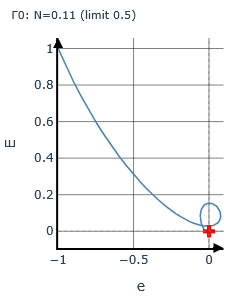
\includegraphics[width=0.325\linewidth]{tuned_F0.png}\hfill
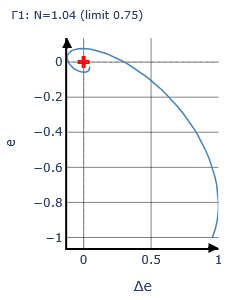
\includegraphics[width=0.325\linewidth]{tuned_F1.png}\hfill

\includegraphics[width=0.325\linewidth]{tuned_F2.png}

\vspace{3mm}
\raggedright
One overshoot, actuator off its limits. Counts
$(3.75,\,4.33,\,4.45) \rightarrow (0.11,\,1.04,\,1.14)$; the residual
lobes are the one-notch cycle at the boundary.
\end{panelbox}

\begin{panelbox}{The gains finding their own way}
\centering

\includegraphics[width=\linewidth]{tuning.png}

\vspace{2mm}
\raggedright
Five halvings settle the diverging start; $K_p, K_i$ come to rest cycling
at the boundary. $K_d$ is walked to the floor --- on this delay-dominated
plant derivative action buys no damping, so \textbf{the tuner returns a
PI controller on its own}.
\end{panelbox}

\begin{panelbox}{Four plants, one set of constants}
\centering
\footnotesize
\setlength{\tabcolsep}{4pt}
\renewcommand{\arraystretch}{2.0}
\begin{tabular}{@{}llcc@{}}
\toprule
& \sffam\bfseries process &
  \sffam\bfseries before &
  \sffam\bfseries after\\
\midrule
P1 & lag-dominant   & $(0.63,\,0.75,\,0.97)$ & $(0.29,\,0.58,\,0.84)$\\
P2 & balanced       & $(0.13,\,\text{-}0.03,\,\textcolor{rust}{1.98})$ & $(0.11,\,0.06,\,0.43)$\\
P3 & delay-dominant & $(0.16,\,0.23,\,\textcolor{rust}{7.48})$ & $(0.09,\,0.74,\,0.87)$\\
P4 & high-order     & $(0.12,\,0.05,\,0.02)$ & $(0.13,\,0.09,\,0.95)$\\
\bottomrule
\end{tabular}

\vspace{4mm}
\raggedright
\normalsize
Nothing in the tuner was adjusted between plants. P4 starts already well
damped, so the run spends itself making it \emph{faster}.
\end{panelbox}

\coltitlebar{6 \; Take home}

\begin{panelbox}{}
\vspace{-5mm}
\begin{itemize}
\item One routine setpoint step per iteration --- the test a technician
      already performs.
\item Dimensionless: the same thresholds for every loop.
\item Names \textbf{the gain and the direction}, not just ``bad''.
\item Every decision is a picture the operator can overrule.
\end{itemize}

\vspace{3mm}
\end{panelbox}

\end{minipage}

\vspace{4mm}
{\color{rule}\rule{\textwidth}{1.6pt}}
\vspace{0.5mm}

\noindent
\begin{minipage}[c]{0.63\textwidth}
{\small\color{muted}Full paper: \emph{Model-Free PID Tuning by Step-Response Inspection} --- D.~Pachner, P.~Otta,
J.~Dost\'al, V.~Havlena. Submitted to \emph{Journal of Process
Control}.}
\end{minipage}\hfill
\begin{minipage}[c]{0.33\textwidth}
\raggedleft
{\small\color{muted}Code, demo and scripts reproducing every number here:
\texttt{github.com/ottapav/roboPID-simulator}}
\end{minipage}

\end{document}
